\documentclass{article}
\usepackage[utf8]{inputenc}
\usepackage{graphicx}
\graphicspath{ {images/} }
\usepackage{algorithm,algorithmic}
\usepackage{amsmath}
\usepackage{amssymb}
\usepackage{mathtools}


\title{GPU based optimizations for large graph adjacency matrices}
\author{Sanjana Garg, 13617}
\date{25 April, 2017}

\begin{document}

\maketitle

\section*{Introduction}
BitMat is a novel compressed bit-vector based index structure previously developed for efficient storage of RDF graph's adjacency matrices. It stores the RDF triples using a 3-dimensional bit-matrix where the three dimensions are subject, object and predicate. A bit is set to $1$ in this matrix if that triple is present. Since, this matrix is sparse, these mats are stored in a compresses format following the D-gap compression scheme.\\

\section*{Motivation}
Fold and unfold are the two primitives in the BitMat system heavily used in the pattern queries for fast operations on the compressed matrices without uncompressing them. Fold and unfold operations operate on each compressed row in a "mutually exclusive" manner using mask bit-vectors (generated by pattern match queries). In this regard, the main contribution of this project is to exploit the "mutual exclusivity" of these operations using the parallelization offered by the GPUs. 

\section*{Fold operation}
The fold operation performs an \textbf{OR} operation over all the rows/columns to give a folded array of the column/row dimension.
Consider an uncompressed bitmat of the following form. Here, the matrix represents the bitmat and the array below that represents the folded array.

\begin{algorithm}[H]
      \begin{algorithmic}[1]
        \FOR {$i = 0$ to $n$}
            \FOR{$j = 0$ to $m$}
                \STATE $foldarr[j] \gets foldarr[j]$ or $BitMat[i][j]$
            \ENDFOR
        \ENDFOR
      \end{algorithmic}
      \caption{CPU\_Fold(BitMat, n, m)}
\end{algorithm}


\begin{figure}[h]
        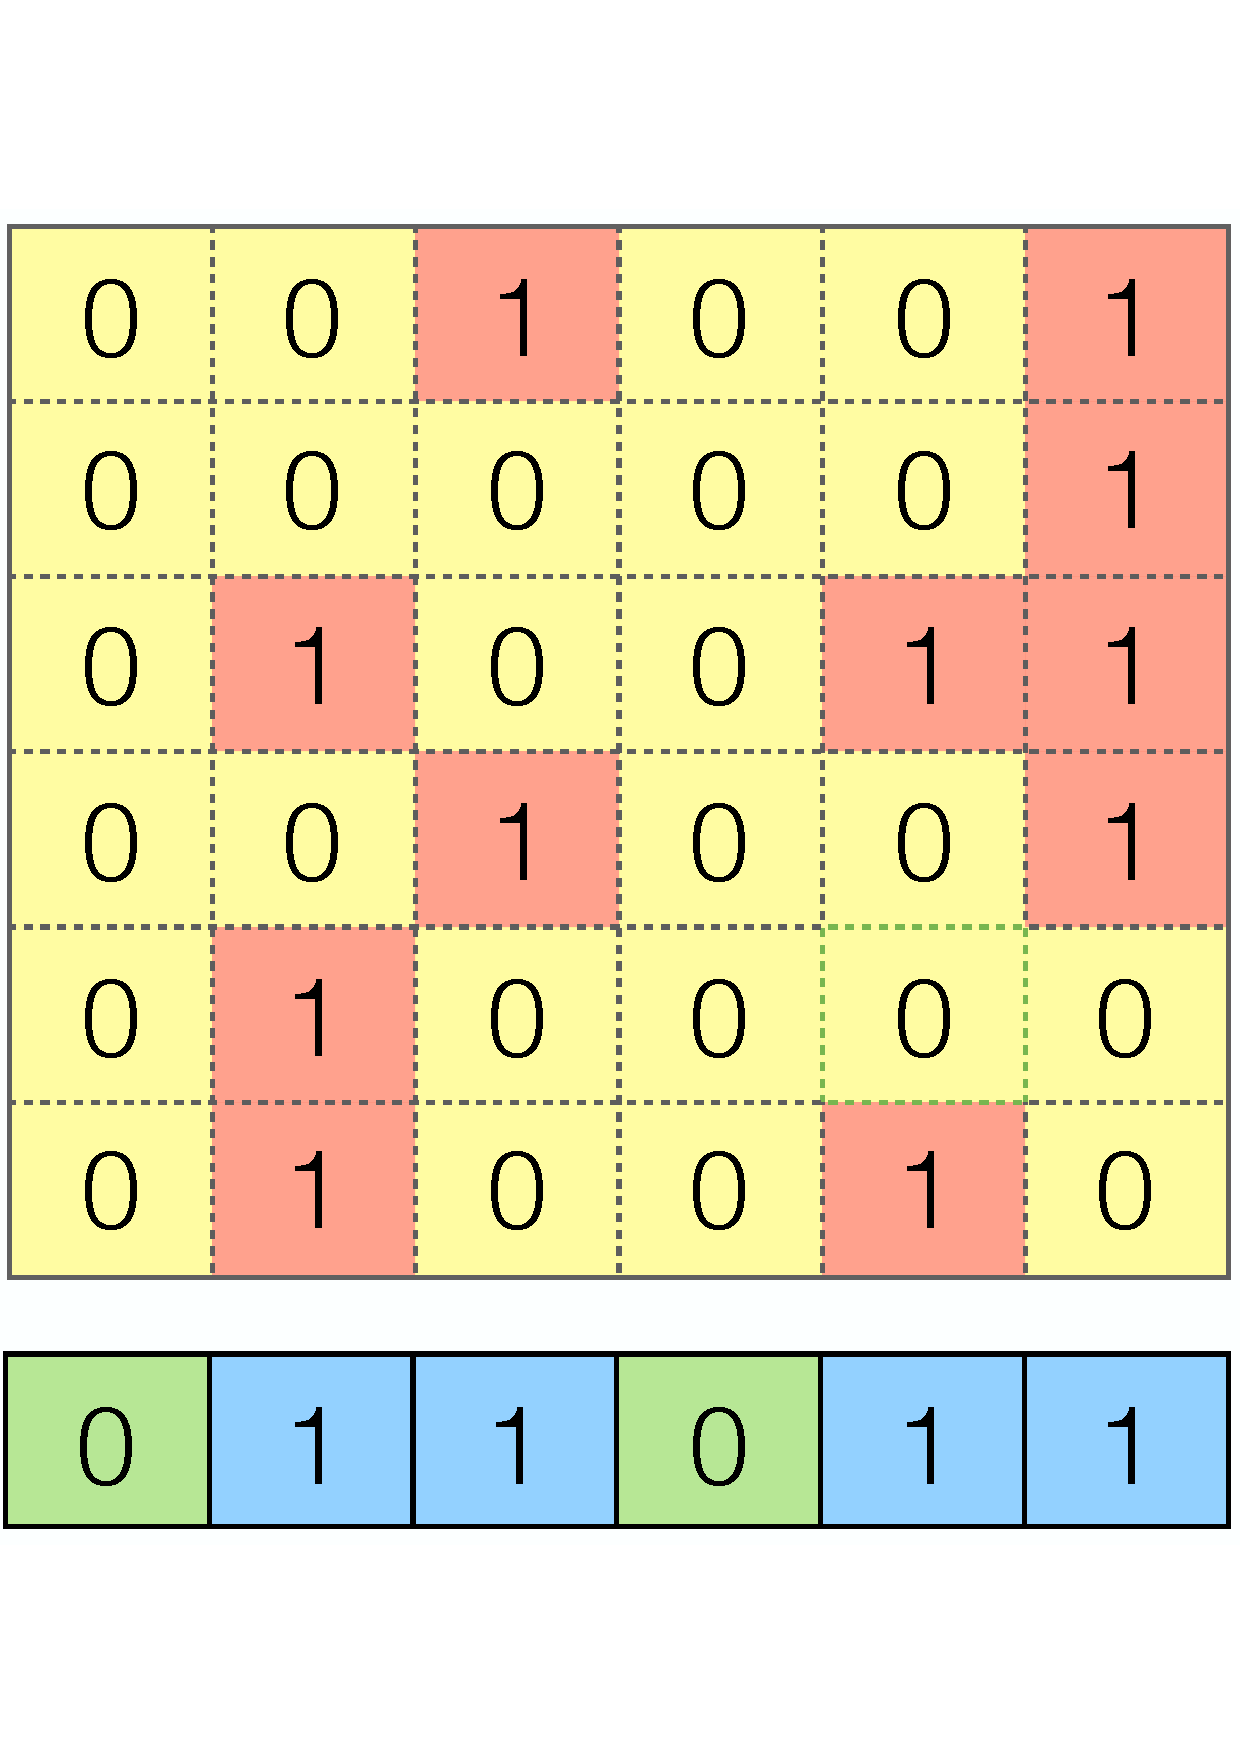
\includegraphics[width=.5\textwidth]{OR.pdf}
        \caption{In this figure, matrix represents an uncompressed BitMat while the array represents the folded array. }
        \centering
\end{figure}

\section*{Unfold operation}
The unfold operation takes as input a bitmat and a mask array and outputs a bitmat with all it's rows ANDed with the mask array.

\begin{algorithm}[H]
      \begin{algorithmic}[1]
        \FOR {$i = 0$ to $n$}
            \FOR{$j = 0$ to $m$}
                \STATE $output[i][j] \gets maskarr[j] \& input[i][j]$
            \ENDFOR
        \ENDFOR
      \end{algorithmic}
      \caption{CPU\_Fold(input, maskarr, output, n, m)}
\end{algorithm}

\begin{figure}[h]
        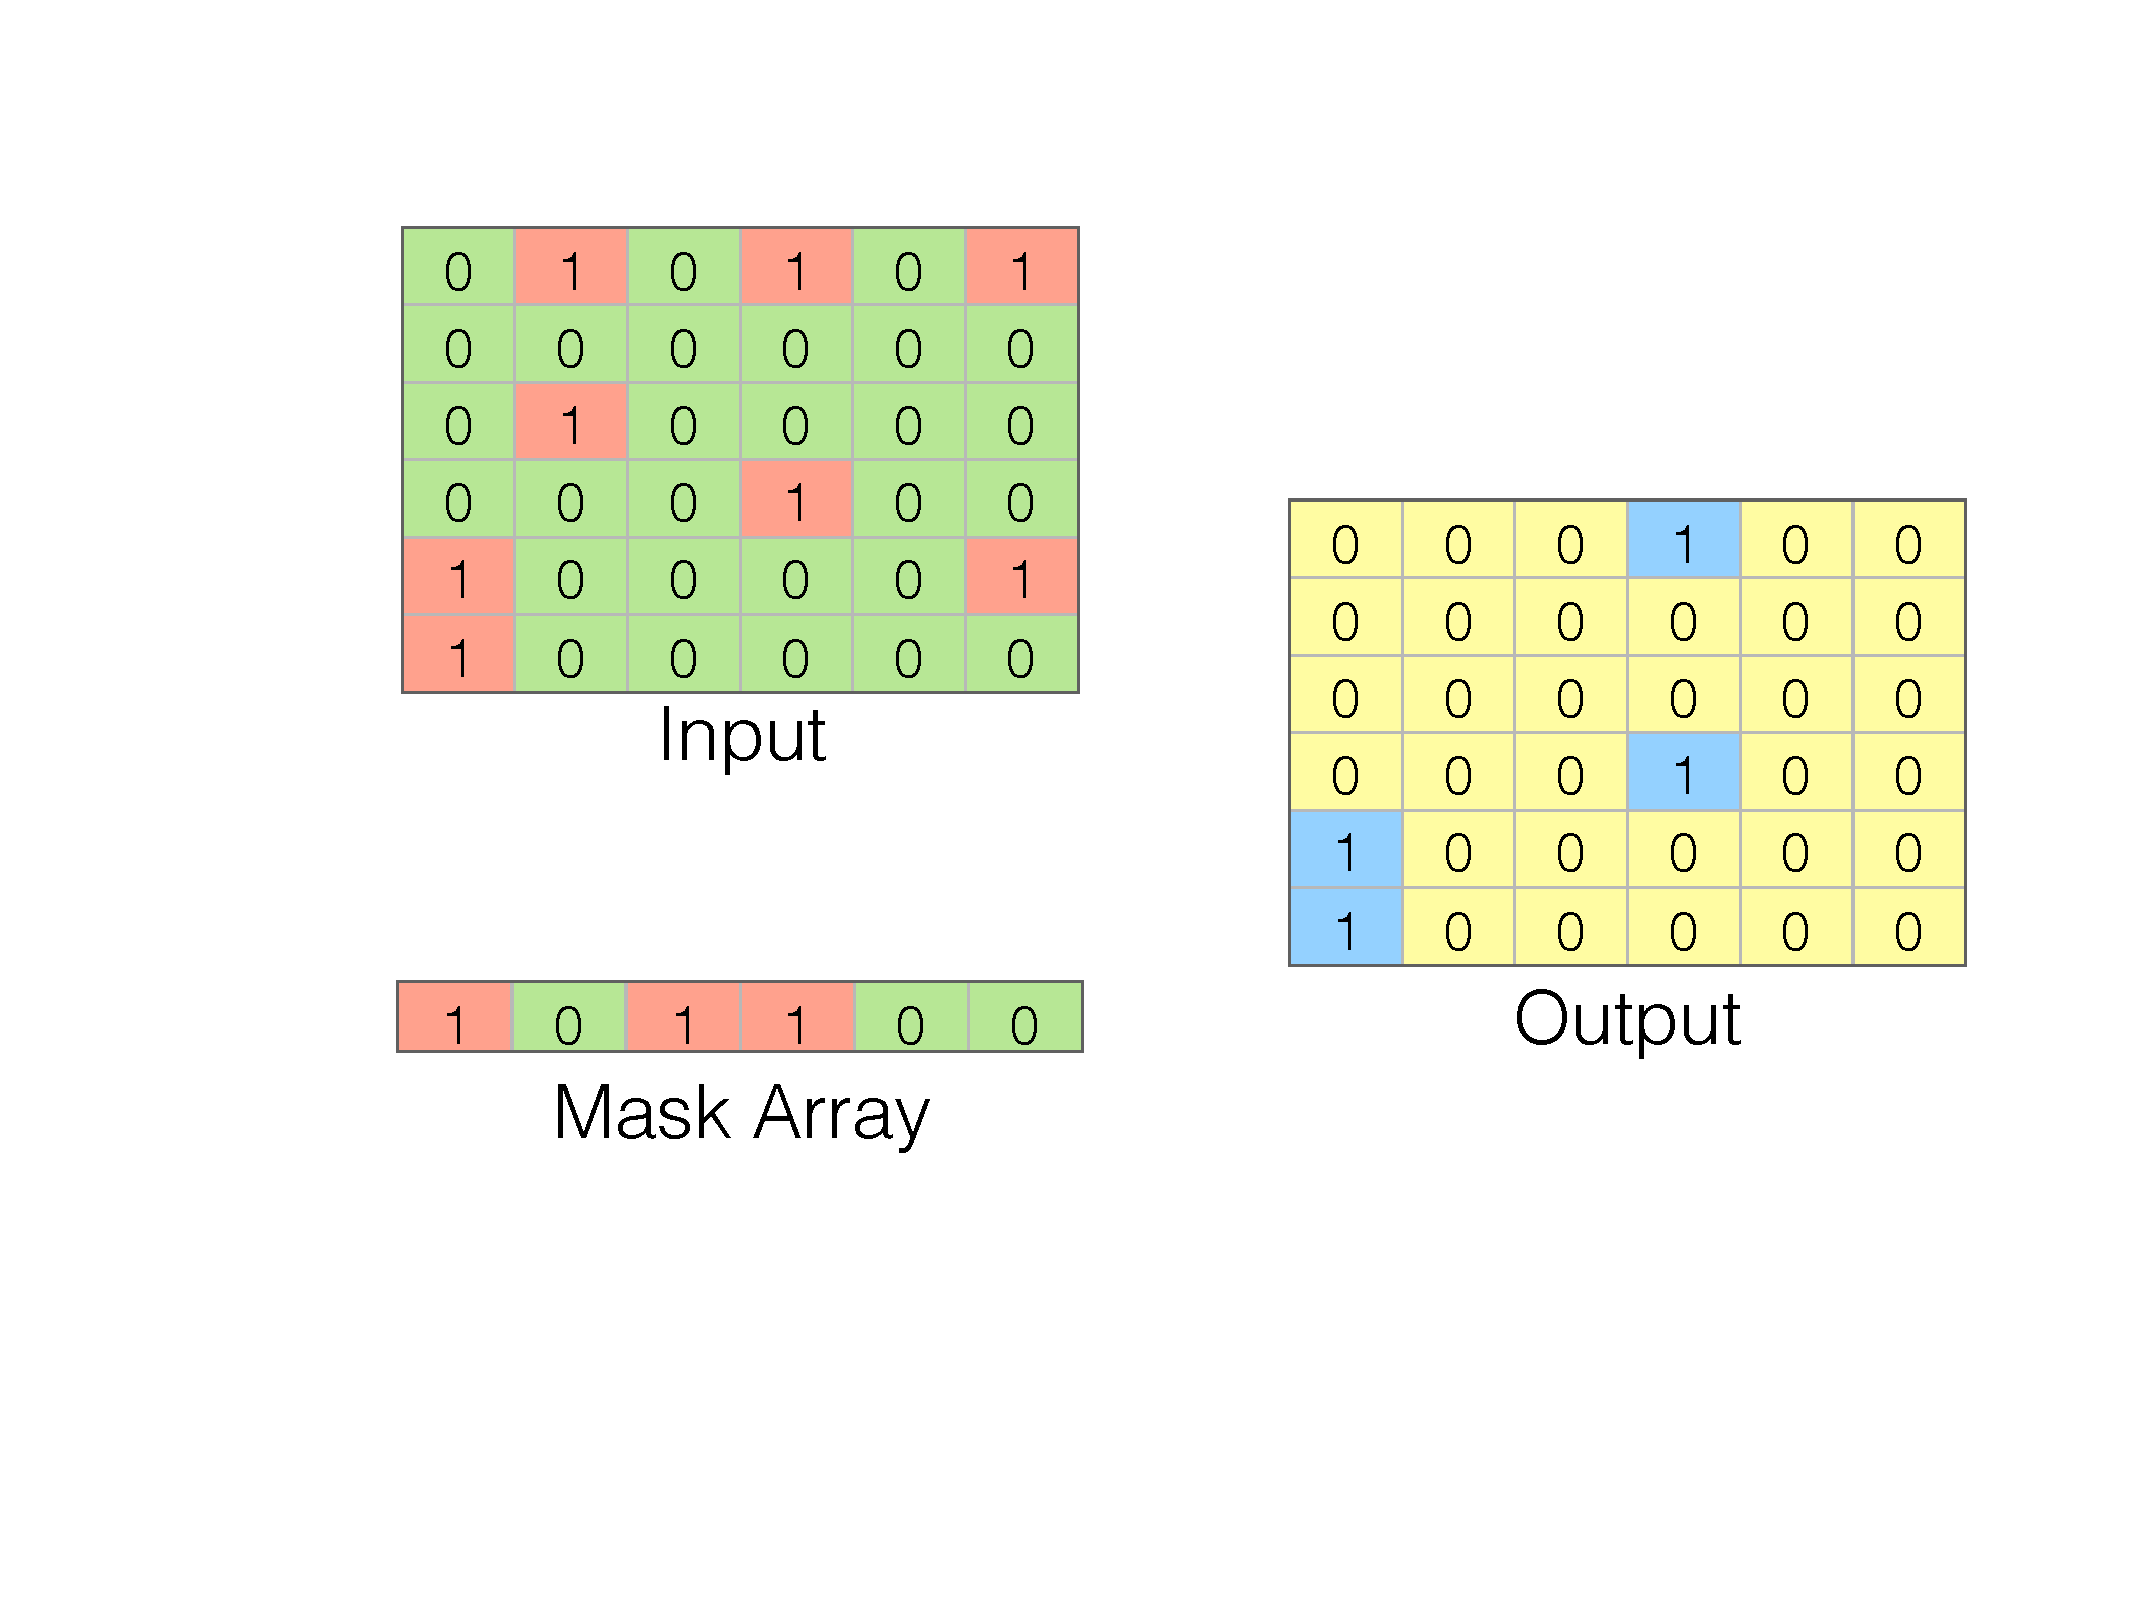
\includegraphics[width=\textwidth]{AND.pdf}
        \caption{In this figure, matrix represents an uncompressed BitMat while the array represents the mask array. Output is the result of applying unfold operation on input as outlined in the algorithm above}
        \centering
\end{figure}

\section*{Parallelization in CUDA}
\subsection*{Architecture}
CUDA is a library developed to exploit the parallelization in GPUs. The architecture divides the code and data into two parts: device and host. Here device, refers to the GPU and host to the CPU machine. The parallelization is performed by threads. The threads are organized into blocks where a block is executed by a multiprocessing unit. The blocks are further organized into a grid. Both the threads and blocks can have a 1, 2 or 3-dimensional index. The grids map to GPUs, blocks to multiprocessors and threads to stream processors.\\

In this project, I have used a 1-dimensional indexing for both threads and blocks as the parallelization is only on 1-dimension int the BitMat, either row or column.

\begin{figure}[h]
        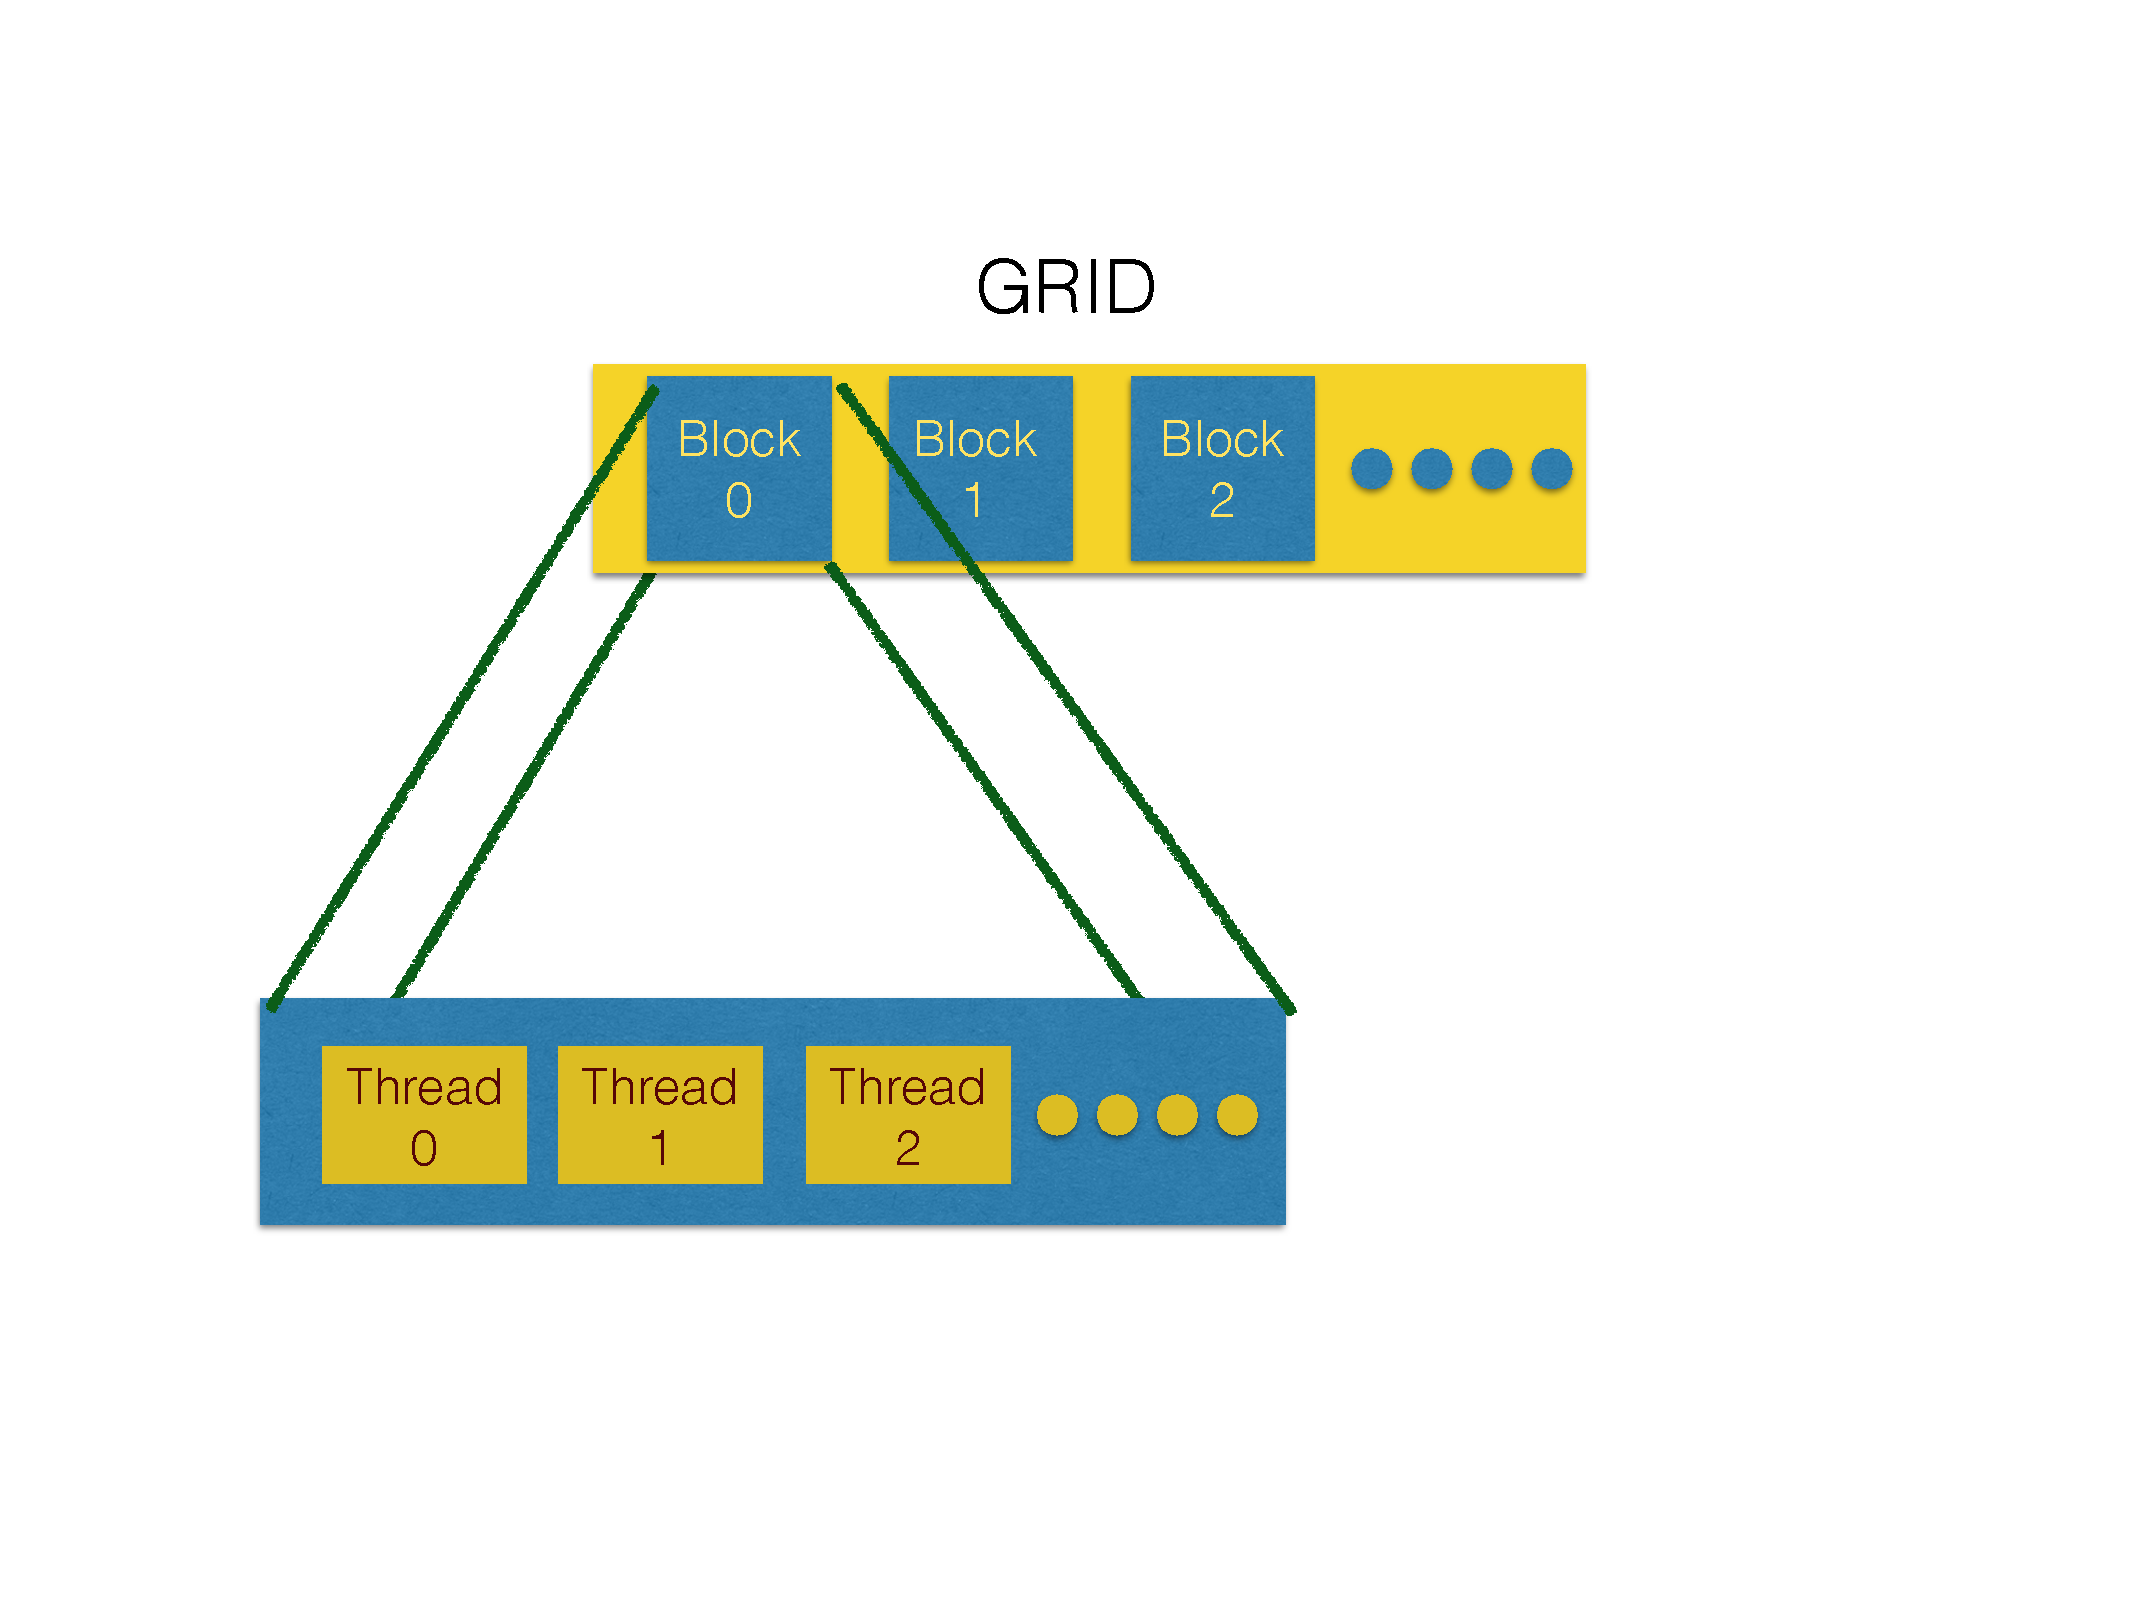
\includegraphics[width=\textwidth]{GPU.pdf}
        \caption{This figure represents the one-dimensional indexing based architecture for both threads and blocks}
        \centering
\end{figure}

\subsection*{Configuration}
Following are the hardware details of the machine used for experimentation
\begin{itemize}
    \item GPU: NVIDIA GeForce GTX 760 2GB
    \item Maximum number of threads per block: 1024
\end{itemize}

Following is the configuration of threads and blocks employed in the project
\begin{align*}
        n &= \text{Number of rows}\\
        split &= \text{Number of rows assigned to a thread}\\
        required\_threads &= ceil(n/split)\\
        numBlocks &= ceil(required\_threads/threadsPerBlock)
\end{align*}


\section*{Parallelized Fold operation}


\end{document}
